%!TEX builder = latexmk
%!TEX program = xelatex
%!TEX option = -shell-escape
\documentclass[oneside,english]{book}
%\ifdefined\directx
%  \usepackage{fontspec}
%\else
%  \usepackage[T1]{fontenc}
%  \usepackage[nomath]{lmodern}
%\fi

\usepackage[T1]{fontenc}
\usepackage[normalem]{ulem}
\usepackage[letterpaper]{geometry}
\geometry{verbose,tmargin=1in,bmargin=1in,lmargin=1in,rmargin=1in}

% table of contents and numbering
\usepackage{tocbibind}
\setcounter{secnumdepth}{3}
\setcounter{tocdepth}{3}

\usepackage{babel}
\usepackage{float}
\usepackage{textcomp}
\usepackage{amsfonts,amsmath,amssymb,mathptmx}
\usepackage{mathrsfs}
\usepackage[colorlinks, citecolor=blue, linkcolor=black, anchorcolor=black]{hyperref}
\usepackage[dvipsnames,usenames]{xcolor}

\usepackage[list=true]{subcaption}

% colors to show the corrections
\definecolor{light-gray}{rgb}{0.7,0.7,0.7}
\definecolor{dark-gray}{rgb}{0.1,0.1,0.3}
\definecolor{light-blue}{rgb}{0.7,0.7,0.9}
\definecolor{dark-blue}{rgb}{0.2,0.2,0.5}

\definecolor{codeblue}{rgb}{0.5,0.5,0.7}
\definecolor{codegreen}{rgb}{0,0.6,0}
\definecolor{codegray}{rgb}{0.5,0.5,0.5}
\definecolor{codepurple}{rgb}{0.58,0,0.82}
\definecolor{backcolour}{rgb}{0.95,0.95,0.92}

%code
\usepackage{listings}
\lstset{
    language=C,
    columns=fixed,       
    frame=no, %tb,                                     
    %backgroundcolor=\color[RGB]{244,244,244},            
    keywordstyle=\color[RGB]{40,40,255},                 
    %numberstyle=\footnotesize\color{darkgray},           
    commentstyle=\it\color[RGB]{0,96,96},                
    stringstyle=\rmfamily\slshape\color[RGB]{128,0,0},   
    showstringspaces=false,                                                          
    basicstyle=\small\ttfamily, %\scriptsize%\tiny%\footnotesize  
    belowcaptionskip=0.5\baselineskip,
    breaklines=true
}

\definecolor{light-gray}{rgb}{0.7,0.7,0.7}
\definecolor{dark-gray}{rgb}{0.1,0.1,0.3}
\definecolor{light-blue}{rgb}{0.7,0.7,0.9}
\definecolor{dark-blue}{rgb}{0.2,0.2,0.5}

\colorlet{punct}{red!60!black}
\definecolor{background}{HTML}{EEEEEE}
\definecolor{delim}{RGB}{20,105,176}
\colorlet{numb}{magenta!60!black}

\lstdefinelanguage{json}{
    basicstyle=\normalfont\ttfamily,
    %numbers=left,
    %numberstyle=\scriptsize,
    %stepnumber=1,
    %numbersep=8pt,
    showstringspaces=false,
    breaklines=true,
    frame=lines,
    backgroundcolor=\color{background},
    literate=
     *{0}{{{\color{numb}0}}}{1}
      {1}{{{\color{numb}1}}}{1}
      {2}{{{\color{numb}2}}}{1}
      {3}{{{\color{numb}3}}}{1}
      {4}{{{\color{numb}4}}}{1}
      {5}{{{\color{numb}5}}}{1}
      {6}{{{\color{numb}6}}}{1}
      {7}{{{\color{numb}7}}}{1}
      {8}{{{\color{numb}8}}}{1}
      {9}{{{\color{numb}9}}}{1}
      {:}{{{\color{punct}{:}}}}{1}
      {,}{{{\color{punct}{,}}}}{1}
      {\{}{{{\color{delim}{\{}}}}{1}
      {\}}{{{\color{delim}{\}}}}}{1}
      {[}{{{\color{delim}{[}}}}{1}
      {]}{{{\color{delim}{]}}}}{1},
}

\IfFileExists{url.sty}{\usepackage{url}}
                      {\newcommand{\url}{\texttt}}

% biblio
\usepackage[authoryear]{natbib}
% biblio GJI
\bibliographystyle{abbrvnat}

% fonts
\usepackage{times}

% figures
\usepackage{graphicx}

\usepackage{enumitem}
\setitemize[1, 2]{topsep=0em, itemsep=0.0em, partopsep=0em, leftmargin=1em}
% we are running pdflatex, so convert .eps files to .pdf
%\usepackage[dvips]{epsfig}


\usepackage{fancyhdr}

\graphicspath{{figure/}}

\setlength{\parskip}{0.4em}
% create thumbnails
%\usepackage[pdftex]{thumbpdf}

%\usepackage{breakurl}

% BibTeX logo
\newcommand{\BibTeX}{{\rm B\kern-.05em{\sc i\kern-.025em b}\kern-.08em{T}\kern-.1667em\lower.7ex\hbox{E}\kern-.125emX}}

%%%%%%%%%%%%%%%%%%%%%%%%%%%%%% Start of document.

\begin{document}


%%%%%%%%%%%%%%%%%%%%%%%%%%%%%%%%%%%%%%%%%%%%%%%%%
%% TITLE page
%%%%%%%%%%%%%%%%%%%%%%%%%%%%%%%%%%%%%%%%%%%%%%%%%
%\begin{center}
%\thispagestyle{empty}\vspace*{-1.8truecm} %
%\makebox[1\textwidth]{%
%\includegraphics[width=0.83\paperwidth]{figures/.pdf} %
%}
%\par\end{center}


\title{\textbf{CGFD3D Seismic Wave Simulation Program}\\
       \textbf{User Manual}}
 

\author{\copyright \, zwlab}

% date of last edit
\date{\today}

\maketitle

%%%%%%%%%%%%%%%%%%%%%%%%%%%%%%%%%%%%%%%%%%%%%%%%%

\newpage{}


%%%%%%%%%%%%%%%%%%%%%%%%%%%%%%%%%%%%%%%%%%%%%%%%%
%% Table of contents
%%%%%%%%%%%%%%%%%%%%%%%%%%%%%%%%%%%%%%%%%%%%%%%%%

\newpage

\tableofcontents

%%%%%%%%%%%%%%%%%%%%%%%%%%%%%%%%%%%%%%%%%%%%%%%%%

%\include{01_introduction}
\chapter{Generation of Computational Grid}\label{chapter-grid}

The computational grid is the basis of the grid-based numerical solver.
The simplest and most easily generated grid is a Cartesian grid (Figure~\ref{fig_grid_cart}), 
whose grid lines are parallel with Cartesian coordinate axes,
thus it can be easily generated by giving the triple value:
the starting point, number of points and the spacing interval.
But the Cartesian grid has difficulty to produce high accurate solution
if there is surface topography in seismic wave simulation.
For surface topography, a general cuvilinear grid system is more accurate (Figure~\ref{fig_grid_curv}).
Its grid lines conform with the surface topography,
thus the surface topography can be accurately represented by the grid.
CGFD3D supports both the Cartesian grid for high efficient simulation
and also the curvilinear grid for high accurate calculation with surface topography.

\begin{figure}[h!]
    \centering
    \subcaptionbox{Cartesian grid\label{fig_grid_cart}}%
        {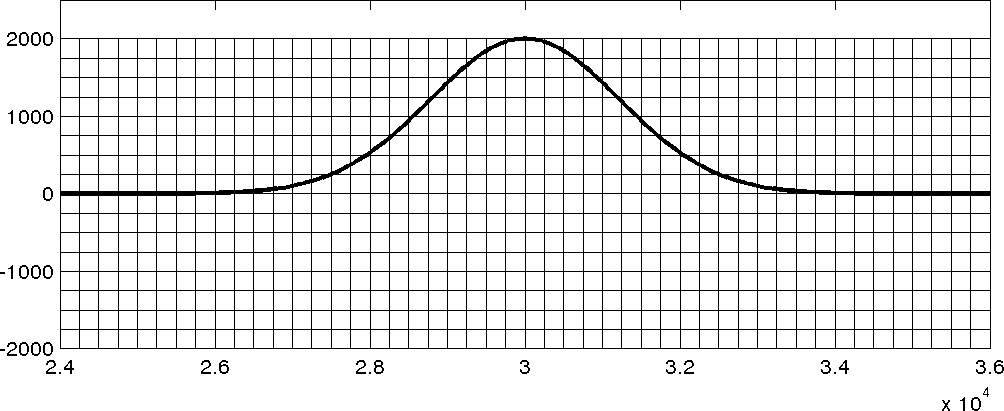
\includegraphics[width=0.4\textwidth]{grid_cart.png}}%
     \hspace{0.1\textwidth}
    \subcaptionbox{Curvilinear grid\label{fig_grid_curv}}%
        {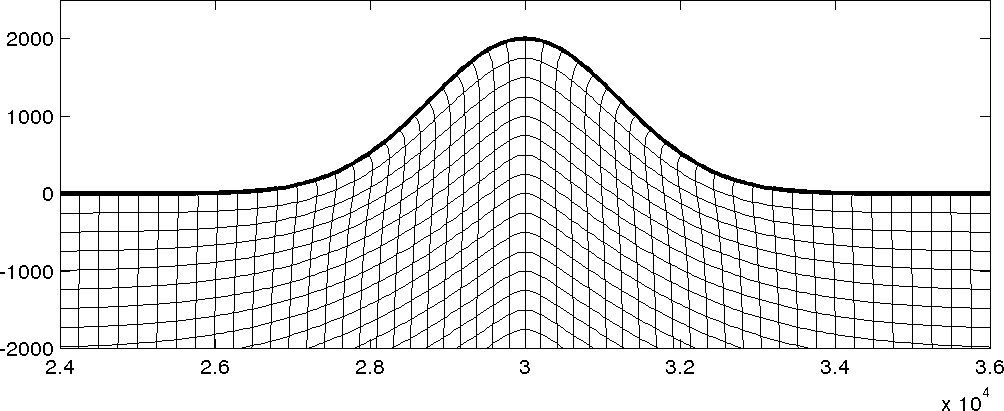
\includegraphics[width=0.4\textwidth]{grid_curv_bold.png}}%
    \caption{Computational grids}
    \label{fig_grid}
\end{figure}

%\begin{figure}
%    \centering
%    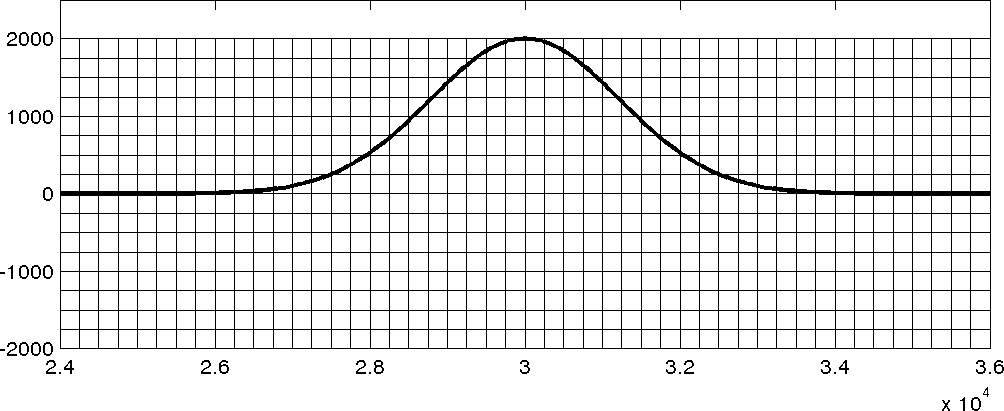
\includegraphics[width=0.5\textwidth]{grid_cart.png}
%    \caption{Cartesian grid with topographic surface plotted as bold line.}
%    \label{fig_grid_cart}
%\end{figure}
%
%%\begin{figure}
%%    \centering
%%    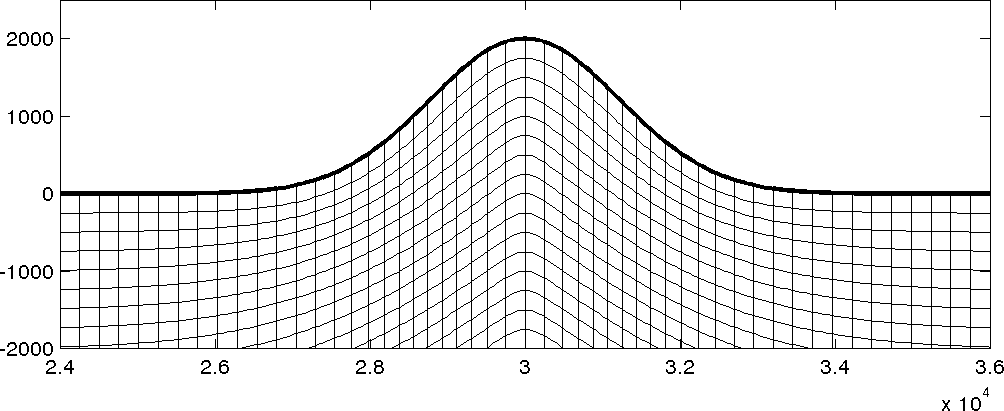
\includegraphics[width=0.5\textwidth]{grid_vmap_bold.png}
%%    \caption{Vertical deformated grid with topographic surface plotted as bold line.}
%%    \label{fig_grid_vmap}
%%\end{figure}
%
%\begin{figure}
%    \centering
%    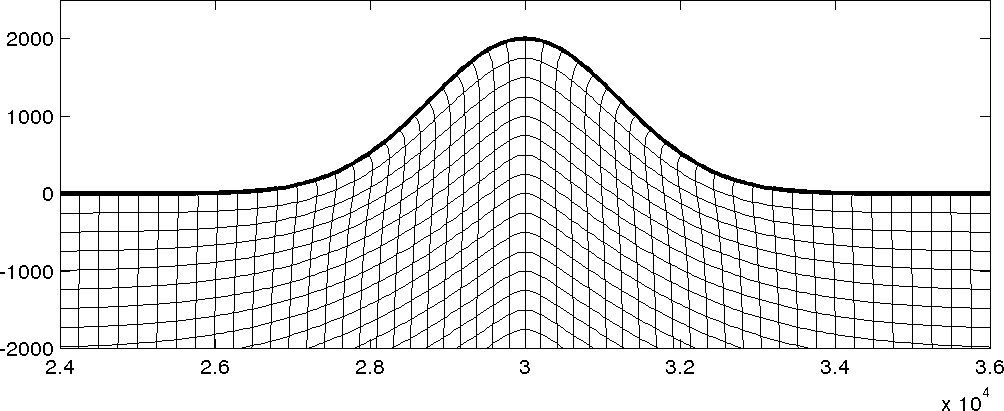
\includegraphics[width=0.5\textwidth]{grid_curv_bold.png}
%    \caption{General curvilinear grid with topographic surface plotted as bold line.}
%    \label{fig_grid_curv}
%\end{figure}


%===============================================================================
\section{Set Grid Parameters in Main Par} \label{sec_grid_json} 
%===============================================================================

\begin{lstlisting}[language=json,
 caption=Grid related parameters in .json,
 label={lst_grid_json},
 frame=tb]
  "grid_generation_method" : {
    "key name" : value
  },
  "is_export_grid" : 1,
  "grid_export_dir"   : "/home/user/prj/output",               
\end{lstlisting}

As shown in List~\ref{lst_grid_json}, user needs to set following parameters
related to the grid in .json file:
\begin{itemize}
  \item \verb|grid_generation_method|: \\
    how the grid is generated.
    There are current three possible methods:

    \begin{itemize}
      \item \verb|import|: \\
        import previoused generated curvilinear grid, 
        thus no need to re-generate grid for repeated run. 
        select this option and give the folder of the exported curvilinear grid, e.g.:  \\
        \verb|"import" : "/home/user/prj/grid"| 

      \item \verb|cartesian|: \\
        generate Cartesian grid, see next section for details.

      \item \verb|layer_interp|: \\
        generate general curvilinear grid, see later section for details.
    \end{itemize}

  \item \verb|is_export_grid|: \\
    if the coordiantes of the curvilinear grid are exported 
         for display purpose or reuse for later calculation without re-generateion of the curvilinear grid.
      \begin{itemize}
        \item 0: do not export,
        \item 1: export.
      \end{itemize}

  \item \verb|grid_export_dir|: \\
    set the output dir if \verb|is_export_grid : 1|.
\end{itemize}

%===============================================================================
\section{Generation of Cartesian Grid} \label{sec_cartesian} 
%===============================================================================

To use the Cartesian grid, we can simply set parameters in the .json file as List~\ref{lst_cart}.
The Cartesian grid needs following parametgers:
\begin{itemize}
  \item \verb|origin|: the x, y and z coordina of the first point,
  \item \verb|interval|: the x, y and z grid spacing. 
\end{itemize}

\begin{lstlisting}[language=json,
 caption={Example of Using Cartesian Grid in .json},
 label={lst_cart},
 frame=tb]
  "grid_generation_method" : {
      "cartesian" : {
        "origin"  : [0.0, 0.0, -5900.0 ],
        "inteval" : [ 100.0, 100.0, 100.0 ]
      }
  },
  "is_export_grid" : 1,
  "grid_export_dir"   : "/home/user/prj/output",               
\end{lstlisting}

%===============================================================================
\section{Generation of General Curvilinear Grid} \label{sec_curv} 
%===============================================================================

We implement a simplified curvilinear grid generation method:
input several topographic grid interfaces as intermidiate interfaces, 
then interpolate grid points between these grid interfaces
with given number of cells between interfaces, which we name as \verb|layer_interp| method.

\begin{lstlisting}[language=json,
 title={Usage Example of \texttt{layer\_interp} in .json},
 label={lst_curv},
 frame=tb]
  "grid_generation_method" : {
      "layer_interp" : {
        "in_grid_layer_file" : "/home/user/prj/input/test_grid.gdlay",  
        "refine_factor" : [ 1, 1, 1 ],
        "horizontal_start_index" : [ 3, 3 ],
        "vertical_last_to_top" : 0
      }
  },
  "is_export_grid" : 1,
  "grid_export_dir"   : "/home/user/prj/output",               
\end{lstlisting}

To use \verb|layer_interp| to generate the curvilinear grid,
we should provide following informations in the .json file (List~\ref{lst_curv}):
\begin{itemize}
  \item \verb|in_grid_layer_file|: \\
    the .gdlay file that represents the curvilinear grid using
      serveral topographic grid interfaces and number of cells between interfaces.
      Please see Section \ref{gridlayerinterp} of the file format description. 
  \item \verb|refine_factor|: \\
      The .gdlay file describes a whole curvinear grid with 
      pre-defined $nx,ny,nz$, number of grid points, and grid spacings.
      If we want to use a smaller grid spacing (denser grid) or larger grid spacing (corser grid),
      we can use this \verb|refine_factor| to change the grid density along different dimensions, e.g.,
      \begin{itemize}
        \item 1: no resampling;
        \item \texttt{2} or \texttt{3}: increase density by two or three times using interpolating;
        \item \texttt{-2} or \texttt{-3}: minus means downsampling by keeping points 
              every two or three points.
      \end{itemize}
      This parameter must be an integer and cannot be zero.
  \item \verb|horizontal_start_index| and \verb|vertical_last_to_top|: \\ 
    We can also use a smaller part of the total .gdlay grid in simulation .
    To do so, we need to tell the program the index of the starting point in the .gdlay to be used.
    Because CGFD3D uses a z-axis positive upward coordinate system, 
    the free surface is located at the end grid size with large number of index of the third dimension.
    Thus we specify the staring points for first and second dimensions through \verb|horizontal_start_index|, 
    while end points of the cut grid to that of the .gdlay through \verb|vertical_last_to_top|.
    E.g.,
    \begin{itemize}
      \item \verb|"vertical_last_to_top" : 0|: \\
          the last layer along 3rd-dim of the cut grid conincides with the free surface in the .gdlay.
      \item \verb|"vertical_last_to_top" : 40|: \\
          the last layer along 3rd-dim of the cut grid conincides with 
            the last 40 points along 3rd-dim in the .gdlay.
    \end{itemize}
    Note: if used with resampling by \verb|refine_factor|,
      there should be at least three points (for current DRP/opt MacCormack scheme) left
          outside the resulting computational grid as the ghost points,
          thus the \\
          \verb|horizontal_start_index| should be set to ensure this condition satisfied, e.g.:
    \begin{itemize}
      \item If you do not resample, the minimum value of \verb|horizontal_start_index| is 3;
      \item If you do two or three times  downsampling,
          the minimum value of \verb|horizontal_start_index| is 6 or 10;
      \item If you do two or three times interpolating,
        the minimum value of \verb|horizontal_start_index| is 2 or 1.
    \end{itemize}
\end{itemize}


%===================================================================
\section{Format of Grid Layer Interp File (.gdlay)} \label{gridlayerinterp}
%===================================================================

\begin{lstlisting}[language=bash,
    numbers=left, numbersep=5pt,numberstyle=\tiny\color{codegray},
    commentstyle=\color{codegreen},
    caption={Example of .gdlay file},
    label={lst_grid_gdlay},
    frame=tb]
     4
     43     10     10
      1      0      1
   126    106
     -300.00      -300.00     -5484.82
     -200.00      -300.00     -5483.59
     -100.00      -300.00     -5481.34
        0.00      -300.00     -5479.30
      100.00      -300.00     -5478.44
      200.00      -300.00     -5478.95
      300.00      -300.00     -5480.11
.
.
.
\end{lstlisting}

\begin{figure}
    \centering
    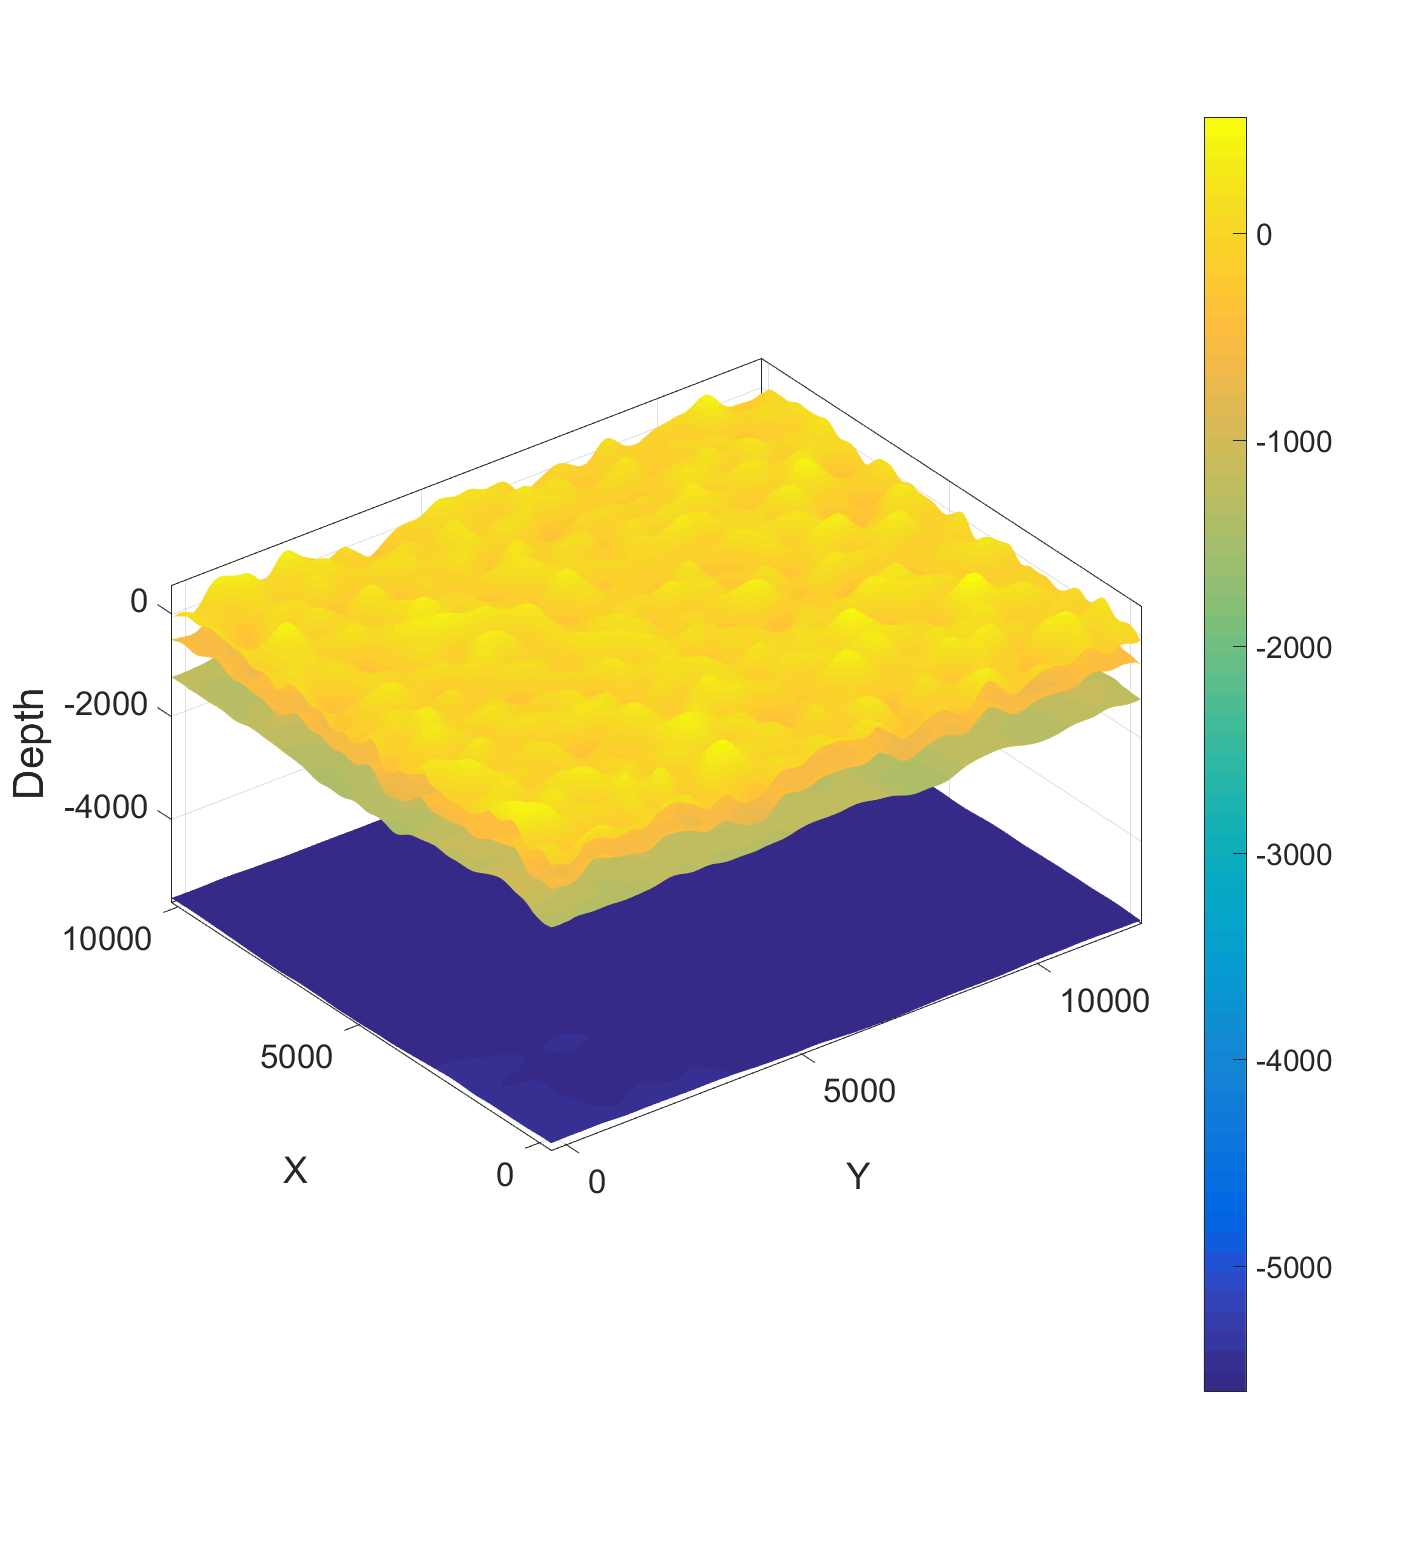
\includegraphics[width=0.8\textwidth]{gdlay_example.png}
    \caption{Examples of the grid interfaces in the .gdlay file.}
    \label{fig_gdlay}
\end{figure}


An example of .gdlay is shown in Listing~\ref{lst_grid_gdlay} and Figure~\ref{fig_gdlay}.
The detailed format of the .gdlay is:
\begin{itemize}
  \item The first line: \\
    the number of grid interfaces ($NI$, 4 in this example).
  \item The second line: \\
    number of cells of each layer
      (the space between two grid interfaces is called a layer).
    There are 43 cells between the 1st and 2nd grid interfaces,
      10 between 2nd and 3rd interfaces,
      10 between 3rd and 4th interfaces in this example.
 \item The third line: \\
   $NI-1$ int values to set if the grid spacing along the 3rd-dim is equal:
   \begin{itemize}
     \item 1: is equal, thus the grid spacing of the 3rd-dim is easily calculated by the two points
         of the grid interfaces in the .gdlay and number of cells of this layer specified in previous line.
     \item 0: not equal or should smoothly vary from 
          the grid spacing of the above grid interfaces to that of lower grid interfaces.
   \end{itemize}
   The variation of the grid spacing between grid layers should be as smooth as possible.
   The vartions of the horizontal grid space is determined by the input grid interfaces in the .gdlay,
    while the variation of the 3rd-dim is affected by values of this line.
   CGFD3D will first generate the grid of the grid layers with equal grid spacing, 
   then generate rest grid between these equal-spacing layers.
   Thus any layer of ``0'' equal value, should have both ``1''  layers above and below it.
  \item The fourth line: \\
    two int values $NX$ and $NY$,
        the number of horizontal grid points of each grid interfaces 
         of this .gdlay file. The numbers are same for all the grid interfaces.
         %thus are given once in this line for all the interfaces.
  \item 
    Rest are the X, Y and Z coordinates of each grid point per line.
    The order of the grid points is:
      1st-dim, then the 2nd-dim of the first grid interface (the bottom one as the z-axis upward positive);
      then those of the 2nd grid interfaces, etc,
    which can can be expressed by the following pseduo code:
\begin{verbatim}
    for (int ilay = 0; ilay < NI; ilay++) {
      for (int j = 0; j < NY; j++) {
        for (int i = 0; i < NX; i++) {
          fscanf(fp,"%g %g %g", &xcoord, &ycoord, &zoord);
        }
      }
    }
\end{verbatim}

\end{itemize}

We provide some examples of matlab scripts to generate .gdlay under the \texttt{example/prep\_grid} directory.

%\subsection{Example}
%
%A model with a horizontal interface can be given as:
%
%\begin{lstlisting}[language=python, title=test.gdlay, frame=tb]
%  4
%  20    10    20
%  1       0     1    
% 100  100
%    100.0    100.0  -5000.0   
%    200.0    100.0  -5000.0
%    300.0    100.0  -5000.0
%    400.0    100.0  -5000.0
%     ...      ...      ... 
%\end{lstlisting}
%The given interface model have 4 interfaces. \\
%There are 20 cells between the first interface and the second interface; there are 10 cells between the second interface and the third interface; there are 20 cells between the third interface and the fourth interface. The first interface is the deepest underground interface, and the last is the free surface interface. \\
%The cell spacing between the first interface and the second interface are equal; the cell spacing between the third interface and the fourth interface are equal; the cell spacing between the second interface and the third interface is gradual.\\
%The number of interface grids in X is 100 and the number of interface grids in Y is 100. The number of interface grids in Z is 51 ( 4+(20-1)+(10-1)+(20-1) ). \\
%
%The given interface model size is \texttt{100*100*51} .
%In fact, the largest model area we can calculate is \texttt{(100-2\*fdx\_nghosts)*(100-2\*fdy\_nghosts)*(51-fdz\_nghosts)}. 
%(In this program, these parameters \texttt{fdx\_nghosts, fdy\_nghosts, fdz\_nghosts} are colonization 3). So the largest model area we can calculate is \texttt{94*94*48}.  \\
%
%(1) Example of the maximum area we can calculate without resampling: \\
%\texttt{number\_of\_total\_grid\_points\_x = 94}, \\
%\texttt{number\_of\_total\_grid\_points\_y = 94}, \\
%\texttt{number\_of\_total\_grid\_points\_z = 48},  \\
%\begin{lstlisting}[language=python, title=run\_test.sh, frame=tb]
%      "layer_interp" : {
%        "in_grid_layer_file" : "$EXEC_DIR/test/test_grid.gdlay",  
%        "refine_factor" : [ 1, 1, 1 ],
%        "horizontal_start_index" : [ 3, 3 ],
%        "vertical_ToFreeSurf_resample_index" : 0
%      }        
%\end{lstlisting}
%the calculation area index range of x is \texttt{3->96}, \\
%the calculation area index range of y is \texttt{3->96}, \\
%the calculation area index range of z is \texttt{3->50}. \\
%In the x direction, ghosts points is \texttt{0->2}, and \texttt{97->99}, \\
%in the y direction, ghosts points is \texttt{0->2}, and \texttt{97->99}, \\
%In the z direction, ghosts points is \texttt{0->2}.\\
%
%(2) Example of the partial area we can calculate without resampling: \\
%\texttt{number\_of\_total\_grid\_points\_x = 50}, \\
%\texttt{number\_of\_total\_grid\_points\_y = 40}, \\
%\texttt{number\_of\_total\_grid\_points\_z = 25}.  \\
%\begin{lstlisting}[language=python, title=run\_test.sh, frame=tb]
%      "layer_interp" : {
%        "in_grid_layer_file" : "$EXEC_DIR/test/test_grid.gdlay",  
%        "refine_factor" : [ 1, 1, 1 ],
%        "horizontal_start_index" : [ 20, 35 ],
%        "vertical_ToFreeSurf_resample_index" : 10
%      }        
%\end{lstlisting}
%the calculation area index range of x is \texttt{20->69}, \\
%the calculation area index range of y is \texttt{35->74}, \\
%the calculation area index range of z is \texttt{16->40}. \\
%In the x direction, ghosts points is \texttt{17->19}, and \texttt{70->72}, \\
%in the y direction, ghosts points is \texttt{32->34}, and \texttt{75->77}, \\
%In the z direction, ghosts points is \texttt{13->15}, and \texttt{41->42}. \\

%number\_of\_total\_grid_points\_x




% !TEX root=./manual_CGFD3D.tex

\chapter{Input Layer or Grid Structure Models}\label{chapter-media}

\markright{CHAPTER \ref{chapter-media} MEDIA}

One major reason to use a computational expensive grid-based seismic wave numerical code
is to simulate seismic wave propagation in complex velocity models,
which can significantly affect the seismic waveforms.
The velocity structure of the Earth, especially near the surface, is vey complex.
How to input the complex velocity model and accurately representing 
the velocity model using the discrete simulation grid are important
components of a seismic wave simulation program.

CGFD3D designs two types of file formats to ease the input of the velocity models.
\begin{itemize}
  \item One is the layer-based model format (.md3lay),
which can be used for topographic layers with known medium paramters along the ingterface and vertical gradients for values inside the layer.
  \item The second one is the grid-based model (.md3grd), which is indeed a hybrid model format that also supports topographic layers structures,
but internal value is interpolated from vertically discrete sampling values inside one layer.
Regular grid models produced by tomography, can be taken as a special case of the .md3grd 
with a single layer and equal vertical invertal at all horizonal sampling points.
\end{itemize}
%support two types of the velocity structure models: layer-based and grid-based.
%The layer-based velocity model can be used for topographic layers 
%  with known medium paramters along the ingterface and vertical gradients for values inside the layer.
%While the grid-based model is indeed a hybrid model format that also supports topographic layers structures,
%but internal value is interpolated from vertically discrete sampling values inside one layer.
%Common grid model, such as results by tomography, 
%The grid-based model 


%===============================================================================
\section{Different Medium Types Supported by CGFD3D} \label{sec_medium_type} 
%===============================================================================

CGFD3D supports simulating wave propagation in following media:
 % TODO: waveform eqn. should be given and analyzed before
\begin{itemize}
    \item \texttt{acoustic\_iso}: abbrevation of acoustic wave equation of isotropic media.  
    \item \texttt{elastic\_iso}: abbrevation of elastic wave equation of isotropic media.
    \item \texttt{elastic\_vti}: abbrevation of elastic wave equation of vertical transversely isotropic media. 
    \item \texttt{elastic\_aniso}: abbrevation of elastic wave equation of anisotropic media. 
\end{itemize}
More complex media will be implemented in the future.

%===============================================================================
\section{Medium Parameterization Methods} \label{equivalent_method} 
%===============================================================================

One parameter the user should determine but the meaning is not so straightfowrad is ``medium parameterization method''.
We explain this concept first to ease description of the medium input in following chapters.

If there are topographic interfaces with strong velocity contrast, 
medium paramters at a grid point directly taking values according to its coordinate in the input velocity model
 will result in stair-case representation of the interfaces, introduce interface-related errors and cause stong artificial diffraction.
One advance feathure of CGFD3D is to evaluate equivalent medium parameters at grid points 
to accurately represent the location of the interface inside a grid cell 
and realize subgrid resolution of the layer velocity models.
CGFD3D supports various medium parameterization approaches:
\begin{itemize}
\item loc: \\
  abbrevation of direct location, which is the simplest and most widely used one. 
      In this approach, the medium parameter of a grid point,
      is the value just at that ccoordinate position
      in the input velocity model. In terms of processing time,
      LOC method is fastest comparing to rest methods.
\item ari: \\
  abbrevation of volume arithmetic averaging as
  \begin{align}
    \left<var\right> = \frac{1}{\Delta V} 
            \int_{k-1/2}^{k+1/2} \int_{j-1/2}^{j+1/2} \int_{i-1/2}^{i+1/2} var~dx dy dz,
  \end{align}
  which evaluats an averaging value for all the medium parameters
    in the cell volume representing by the grid point.
\item har: \\
  abbrevation of volume harmonic averaging for medium modulus as 
  \begin{align}
    \left<var\right>^H = \frac{\Delta V}
      {\int_{k-1/2}^{k+1/2} \int_{j-1/2}^{j+1/2} \int_{i-1/2}^{i+1/2} \frac{1}{var} dx dy dz},
  \end{align}
  which evaluats an averaging value of medium modulus in the cell volume representing by the grid point,
  while and volume arithmetic average for density as proposed by \citet{moczo_3d_2002,moczo_finite-difference_2014}.
  The approach does not alter medium type,
    e.g., isotropic model is still an isotropic one, after parametrization.
\item tti: \\
  abbrevation of tiled transversely isotropic equivalent medium approach \citep{jiang2021tti}, 
        which evaluats an effictive TTI representation of the thin layers inside the cell volume representing by the grid point.
        The approach does alter medium type, e.g., isotropic model becomes a TTI anisotropic one, after parametrization.
\end{itemize}


The parametrization name may mean a slightly different combination of hormonic and arithmetic
averaging of difference medium parameters for different medium types (Table~\ref{table_parameterization}).

\begin{table}[h!]
\centering
\begin{tabular}{| c | c | c | c | c |}
\hline
   medium type               &   loc$^L$   &   ari$^A$   & har$^H$  & tti$^T$ \\
\hline
   \verb|one_component|      &    all$^L$  &   all$^A$   & all$^H$  &  NA \\
\hline
   \verb|acoustic_isotropic| &    all$^L$  &   all$^A$   &$\kappa^H$, $\rho^A$ & NA \\
\hline
   \verb|elastic_isotropic|  &    all$^L$  &   all$^A$   &$\lambda^H$,$\mu^H$,$\rho^A$ &  todo \\
\hline
   \verb|elastic_vti_*|      &    all$^L$  &   all$^A$   &$C_{ij}^H$, $\rho^A$ & todo \\
\hline
   \verb|elastic_aniso_cij|  &    all$^L$  &   all$^A$   &$C_{ij}^H$, $\rho^A$ & todo \\
\hline
   \verb|elastic_tti_*|      &    all$^L$  &   all$^A$   &$C_{ij}^H$, $\rho^A$ & todo \\
\hline
\end{tabular}
\caption{Medium parameterization on difference parameters for different medium types.}
\label{table_parameterization}
\end{table}

%\begin{table}[h!]
%\centering
%\caption{Medium parameterization on difference parameters for different medium types.}
%\label{table_parameterization}
%\begin{tabular}{| c | c | c | c | c | c |}
%\hline
%   medium type  &   \verb|one_component|    &   \verb|acoustic_isotropic| & \verb|elastic_isotropic|
%                &  \verb|elastic_vti_*| & \verb|elastic_aniso_cij/elastic_tti_*| \\
%\hline
%    loc    &   as is  &  as is  &     as is  &     as is  &     as is  \\
%\hline
%  ari$^A$  &   as is  &  as is  &     as is  &     as is  &     as is  \\
%\hline
%   har$^H$ &   as is &  $\kappa^H$, $\rho^A$  &  $\lambda^H$,$\mu^H$,$\rho^A$
%             &     $C_{ij}^H$, $\rho^A$  &  $C_{ij}^H$, $\rho^A$  \\
%\hline
%  tti      &   NA &   NA &   NA &   NA &   NA \\
%\hline
%\end{tabular}
%\end{table}


%If the media type in the \textbf{md3grd} or \textbf{md3lay} file is \texttt{one\_component}, \texttt{equivalent\_medium\_method} can be
%\begin{itemize}
% \item \texttt{loc}: using local value to discrete model. 
% \item \texttt{ari}: volume integral arithmetic average. 
% \item \texttt{har}: volume integral harmonic average, 
%\end{itemize}
%
%If the media type is \texttt{acoustic\_isotropic}, \texttt{equivalent\_medium\_method} can be
%\begin{itemize}
% \item \texttt{loc}: using local media parameters to discrete model. 
% \item \texttt{har}: applying harmonic average to $\kappa$, and applying arithmetic average to density $\rho$. 
% \item \texttt{ari}: applying arithmetic average to $\kappa$ and $\rho$. 
%\end{itemize}
%
%If the media type is \texttt{elastic\_isotropic}, \texttt{equivalent\_medium\_method} can be
%\begin{itemize}
% \item \texttt{loc}: using local media parameters to discrete model. 
% \item \texttt{har}: applying harmonic average to elastic modulus, and applying arithmetic average to density $\rho$. Please see \citet{moczo_3d_2002} and \citep{moczo_finite-difference_2014} for detail.
% \item \texttt{ari}: applying arithmetic average to elastic modulus and density. 
%\end{itemize}
%
%If the media type is \texttt{elastic\_vti\_*}, \texttt{equivalent\_medium\_method} can be
%\begin{itemize}
% \item \texttt{loc}: using local media parameters to discrete model. 
% \item \texttt{har}: applying harmonic average to elastic modulus $c_{ij}$, and applying arithmetic average to density $\rho$.
% \item \texttt{ari}: applying arithmetic average to elastic modulus $c_{ij}$ and density. 
%\end{itemize}
%
%If the media type is \texttt{elastic\_aniso\_cij} or \texttt{elastic\_tti\_*}, \texttt{equivalent\_medium\_method} can be
%\begin{itemize}
% \item \texttt{loc}: using local media parameters to discrete model. 
% \item \texttt{har}: applying harmonic average to elastic modulus $c_{ij}$, and applying arithmetic average to density $\rho$.
% \item \texttt{ari}: applying arithmetic average to elastic modulus $c_{ij}$ and density. 
%\end{itemize}

%===============================================================================
\section{Parameters in Main Par File} \label{sec_medium_json} 
%===============================================================================

\begin{lstlisting}[language=json,
    label={lst_medium_json},
    caption=Example of medium settings in .json,
    frame=tb]
  "medium" : {
      "type" : "elastic_iso",
      "#code" : 1,
      "infile_layer" : "/home/usr1/testCGFD3D/prep_medium/basin.md3lay",
      "#infile_grid" : "/home/usr1/testCGFD3D/prep_medium/basin.md3grd",
      "#equivalent_medium_method" : "har",
      "#import" : "/home/usr1/testCGFD3D/output/media"
  },
  "is_export_media" : 1,
  "media_export_dir"  : "/home/usr1/testCGFD3D/output/media",

  "#visco_config" : {
      "type" : "graves_Qs",
      "Qs_freq" : 1.0
  }
\end{lstlisting}

There are several medium related keys in the main par .josn file (List~\ref{lst_medium_json}),
\begin{itemize}
\item \verb|medium|: \\
  major block for medium input, tells the program:
  \begin{itemize}

  \item \texttt{type} determins the solver equation, that is,
    what medium you want to simulate wave propagation in.
    Four options are currently supported in this code:
    \begin{itemize}
      \item \texttt{acoustic\_iso}: acoustic wave equation of isotropic media,
      \item \texttt{elastic\_iso}: elastic wave equation of isotropic media,
      \item \texttt{elastic\_vti}: elastic wave equation of vertical transversely isotropic media,
      \item \texttt{elastic\_aniso}: elastic wave equation of anisotropic media. 
    \end{itemize}

  \item how the structure model is input or specified.
    There are four possible ways:
    \texttt{import}, \texttt{code}, \texttt{infile\_layer} or \texttt{infile\_grid}.
    \begin{itemize}  
      \item \texttt{code}: \\
        Choose this flag if you want to give the media by code.
                 You should edit \textbf{forward/md\_t.c} file and recompile the code.
      \item \texttt{infile\_layer}: \\
        If you want to give media by the intereface line,
          this option should be helpful. The media parameters are given by the \textbf{md3lay} file,
          and the file format is shown in Section \ref{md3lay} 
      \item \texttt{infile\_grid}: \\
        If you want to give media by a given grid media,
          this option should be helpful. The media parameters are given by the \textbf{md3grd} file,
          the file format is shown in Section \ref{md3grd}.
      \item \texttt{import}: \\
        If you already generated media from the above three options,
        and do not want to re-generate media, 
        select this option and give the folder of the exported media. 
    \end{itemize}

  \item \texttt{equivalent\_medium\_method}: If you specify structure mode by
        \texttt{infile\_layer} or \texttt{infile\_grid},
        equivalent medium parameterization methods can be applied.
        For different media, we provide different equivalent medium parameterization methods,
        please see Section \ref{equivalent_method} for detail.
  \end{itemize}
   
\item \verb|is_export_media|: \\
  if the discreted medium parameters at FD grid points are exported 
       for display purpose or reuse for later calculation without re-discrete media calculation.
    \begin{itemize}
      \item 0: do not export discrete media,
      \item 1: export discrete media.
    \end{itemize}
\item \verb|media_export_dir|: \\
  set the output dir if \verb|is_export_media : 1|.
  
\item \verb|visco_config|: \\
  block for attuantion settings.
  If this block is enabled (appeared in the .json),
    the attuation will be implemented with following two parameters (add Grave's ref):
  \begin{itemize}
    \item \verb|type|: currently only \verb|graves_Qs| can be set, which means to implement
       attuation following Grave (1996) approach.
     \item \verb|Qs_freq|: the frequency of the wavefield for which 
          the Q effect is most accurately approximated.
  \end{itemize}

\end{itemize}


%===================================================================
\section{Format of Layer-based Velocity Model (.md3lay)} \label{md3lay}
%===================================================================

The Earth structure of many regions has following features:
\begin{itemize}
  \item the structure consists of many layers with topographic interfaces,
  \item the velocity or density in some layers may increase or decrease along depth,
      which may be expressed by the value at the interface
      and two polynomial parameters (coefficient and power) with respect to depth.
\end{itemize}
For such structures, we can use .md3lay file to input the structure into CGFD3D.


\begin{lstlisting}[language=bash, caption=Example of .md3lay file,
   numbers=left, numbersep=5pt,numberstyle=\tiny\color{codegray}, commentstyle=\color{codegreen},
    label={lst_medium_md3lay},
   frame=tb]
# media type
elastic_isotropic
# number of interfaces (NI)
4
# NX  NY    X0    Y0    DX    DY   (interface mesh)
 126 106 -300.0 -300.0 100.0 100.0
# elevation  rho   rho_grad rho_pow    vp   vp_grad  vp_pow    vs    vs_grad  vs_pow
   0.0      1000.0    0.2    1.0     1500.0    0.2    1.0     1000.0    0.2    1.0
   0.0      1000.0    0.2    1.0     1500.0    0.2    1.0     1000.0    0.2    1.0
   0.0      1000.0    0.2    1.0     1500.0    0.2    1.0     1000.0    0.2    1.0
   0.0      1000.0    0.2    1.0     1500.0    0.2    1.0     1000.0    0.2    1.0
   0.0      1000.0    0.2    1.0     1500.0    0.2    1.0     1000.0    0.2    1.0
   0.0      1000.0    0.2    1.0     1500.0    0.2    1.0     1000.0    0.2    1.0
   0.0      1000.0    0.2    1.0     1500.0    0.2    1.0     1000.0    0.2    1.0
   .
   .
   .
\end{lstlisting}

\begin{figure}
    \centering
    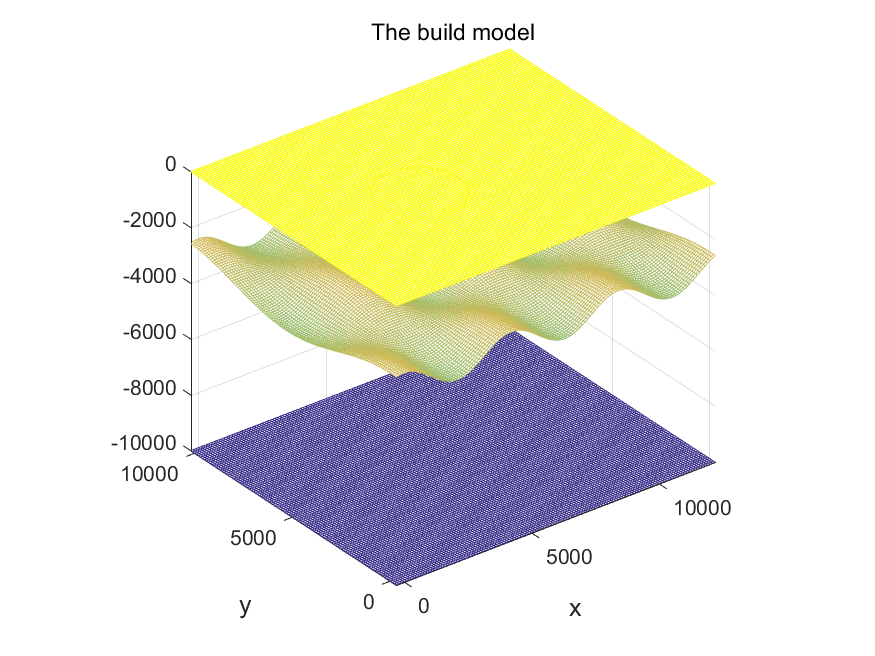
\includegraphics[width=0.5\textwidth]{md3lay_basin.png}
    \caption{Layer-based velocity model with topographic internal interfaces.}
    \label{fig_md3lay}
\end{figure}


An example of .md3lay is shown in Listing~\ref{lst_medium_md3lay} and Figure~\ref{fig_md3lay}.
The detailed format of the .md3lay is:
\begin{itemize}
  \item The first line: sets the medium type, which can be
    \begin{itemize}
    \item \verb|one_component|: \\
      there is only a single medium parameter in this file.
    \item \verb|acoustic_isotropic|: \\
      two parameters $\rho$ and Vp.
    \item \verb|elastic_isotropic|: \\
      three parameters $\rho$, Vp, Vs.
    \item \verb|elastic_vti_prem|: \\
      density and five VTI parameters same to PREM model,
       $\rho$, vph, vpv, vsh, vsv, $\eta$. Please see \citep{dziewonski1981preliminary} for detail.
    \item \verb|elastic_vti_thomsen|: \\
      density and five Thomsen parameters,
        $\rho$, $\alpha_0$, $\beta_0$, $\epsilon$, $\delta$, $\gamma$.
        Please see \citep{ thomsen1986weak} for detail.
    \item \verb|elastic_vti_cij|: \\
      density and five VTI parameters given by $C_{ij}$,
         $\rho$, $c_{11}$, $c_{33}$, $c_{55}$, $c_{66}$, $c_{13}$. 
    \item \verb|elastic_tti_thomsen|: \\
      density ,five Thomsen parameters, two angle of symmetric axis.
         $\rho$, $\alpha_0$, $\beta_0$, $\epsilon$, $\delta$, $\gamma$, $\Phi$, $\theta$.
         Please see \citep{thomsen1986weak} for detail.
    \item \verb|elastic_tti_bond|: \\
          $\rho$, $c_{11}$, $c_{33}$, $c_{55}$, $c_{66}$, $c_{13}$, $\Phi$, $\theta$.
          $\Phi$ is azimuth angle, $\theta$ is the dip angle.
    \item \verb|elastic_aniso_cij|: \\
           $\rho$, $c_{11}$, $c_{12}$, $c_{13}$, $c_{14}$, $c_{15}$, $c_{16}$,  
                                      $c_{22}$, $c_{23}$, $c_{24}$, $c_{25}$, $c_{26}$, 
                                      $c_{33}$, $c_{34}$, $c_{35}$, $c_{36}$, $c_{44}$,
                                      $c_{45}$, $c_{46}$, $c_{55}$, $c_{56}$, $c_{66}$.

    \end{itemize}

  \item The second line: the number of interface (\texttt{NI}) (4 in this example).

  \item The third line:
    six values (two integers and four float) specify the horizontal sampling points as:\\
    \texttt{NX} ~~ \texttt{NY} ~~ \texttt{X0} ~~ \texttt{Y0} ~~ \texttt{DX} ~~ \texttt{DY}, \\
    where
    \begin{itemize}
      \item \texttt{NX} and \texttt{NY}:
          the number of sampling points along $x$ and $y$ direction (126 and 106 for this example);
      \item \texttt{X0} and \texttt{Y0}: 
        the $x$ and $y$ coordinates of the first point (-300.0 and -300.0 for this example);
      \item \texttt{DX} and \texttt{DY}:
        spacing between sampling points along $x$ and $y$ (100.0 and 100.0 for this example).
    \end{itemize}

 \item 
  Rest are the elevation and media parameters of each sampling point per line.
  Take the \texttt{elastic\_isotropic} media as an example, the media parameters are read as:
  \begin{lstlisting}[language = C]
  for (ni=0; ni<NI; ni++)
    for (iy=0; iy<NY; iy++) 
      for (ix=0; ix<NX; ix++) 
        fscanf(in_3lay_file, "%f %f %f %f %f %f %f", 
               &elevation,
               &rho, &rho_grad, &rho_pow,
               &vp, &vp_grad, &vp_pow,
               &vs, &vs_grad, &vs_pow);
  \end{lstlisting}
  where \texttt{*\_grad} and \texttt{*\_pow} are the coefficient and power of the parameters
    in z-direction as in following equation:
   \begin{equation*}
     \rm{value}^{\rm{grid~point}} = \rm{value}^{\rm{interface}}
        + (z^{\rm{interface}}-z^{\rm{grid~point}})^{var\_pow} * var\_grad.
   \end{equation*}
   Please notice that the z-axis is positive upward in CGFD3D.

\end{itemize}

Please note that
\begin{itemize}
  \item if the computational grid point is located above the top interface of the .md3lay model,
the medium parameters are taken as the values at the top interface.
  \item Different media parameters can have different \texttt{*\_grad} and \texttt{*\_pow}.
\end{itemize}

You can find matlab example script to generate .md3lay in \textbf{example/prep\_medium} directory.

%===================================================================
\section{Format of Grid-based Velocity Model (.md3grd)} \label{md3grd}
%===================================================================

If the velocity variation along depth inside a layer can not be expressed by a polynomial expression
with respect to depth, then we have to give sampling values at discrete points along the depth.
This is why we privoide the .md3grd, the grid-based velocity file.

We design the .md3grd also supporting layer interfaces,
thus the interface effects can be simulated as accurate as possible.
To do so, we need to also set number of layers in the .md3grd file,
then discrete the velocity variation along depth for each layer.


\begin{lstlisting}[language=bash, caption=Example of .mdgrd file,
   numbers=left, numbersep=5pt,numberstyle=\tiny\color{codegray}, commentstyle=\color{codegreen},
    label={lst_medium_md3grd},
   frame=tb]
# media type   
elastic_isotropic
# number of layers (NL)
3
# number of grids in the z-direction for each layer of the NL layers
 11 21 101
# NX  NY  X0     Y0    DX    DY    (mesh in xOy of the given model)
126 106 -300.0 -300.0 100.0 100.0
# elevation  rho     vp      vs  
   0.0      1000.0  1510.0  1020.0
   0.0      1000.0  1510.0  1020.0
   0.0      1000.0  1510.0  1020.0
   0.0      1000.0  1510.0  1020.0
   0.0      1000.0  1510.0  1020.0
   0.0      1000.0  1510.0  1020.0
   0.0      1000.0  1510.0  1020.0
   .
   .
   .
\end{lstlisting}

%\begin{figure}
%    \centering
%    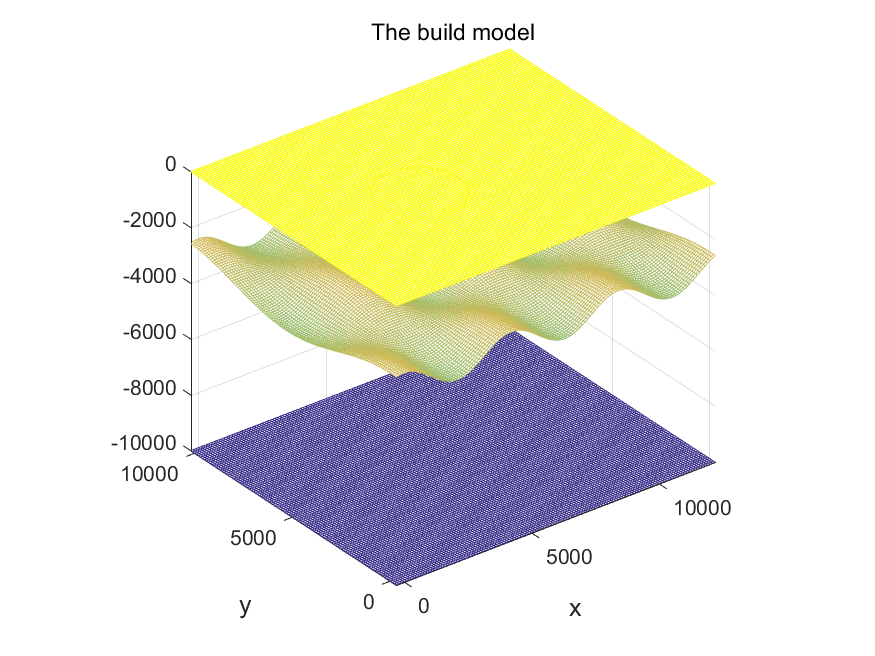
\includegraphics[width=0.5\textwidth]{md3lay_basin.png}
%    \caption{Layer-based velocity model with topographic internal interfaces.}
%    \label{fig_md3grd}
%\end{figure}


An example of .md3grd is shown in Listing~\ref{lst_medium_md3grd}. % and Figure~\ref{fig_md3grd}.
The detailed format of the .md3grd is:
\begin{itemize}
  \item The first line: \\
    sets the medium type, similar to that of .md3lay. 
     Please see descriptions in \ref{md3lay}.

   \item The second line: \\
     is the number of layer or interfaces (\texttt{NL}) (3 in this example).
     If \texttt{NL} = 1, the model becomes the standard grid model that
     only has descrete sampling value along depth but without interfaces.
     If \texttt{NL} > 1, the equivalent medium parameterization can be applied across the interfaces.

   \item The next \texttt{NL} numbers (either at the same line or \texttt{NL} lines)
     set the number of grids in the z-direction of \texttt{NL} layer.
  
   \item The next line: \\
      six values (two integers and four float) specify the horizontal sampling points as:\\
      \texttt{NX} ~~ \texttt{NY} ~~ \texttt{X0} ~~ \texttt{Y0} ~~ \texttt{DX} ~~ \texttt{DY}, \\
      where
      \begin{itemize}
        \item \texttt{NX} and \texttt{NY}:
            the number of sampling points along $x$ and $y$ direction (126 and 106 for this example);
        \item \texttt{X0} and \texttt{Y0}: 
          the $x$ and $y$ coordinates of the first point (-300.0 and -300.0 for this example);
        \item \texttt{DX} and \texttt{DY}:
          spacing between sampling points along $x$ and $y$ (100.0 and 100.0 for this example).
      \end{itemize}

  \item Rest are the elevation and media parameters of every grid point per line.
    Take the \texttt{elastic\_isotropic} media as an example,
    the media parameters are read as:
  \begin{lstlisting}[language = C]
  for (nl=0; nl< NL; nl++)
    for (ip=0; ip<np[nl]; np++)
      for(iy=0; iy<NY; iy++)
        for (ix=0; ix<NX;ix++)
          fscanf(in_3grd_file, "%f %f %f %f", 
              &elevation, &rho, &vp, &vs);
  \end{lstlisting}
  The medium parameter at a computational grid point is calculated
    by linear interpolation of two values at the discrete velocity model points
    nearest to the computational grid point.

\end{itemize}


Please note that
\begin{itemize}
  \item if the computational grid point is located above the top interface of the .md3grd model,
the medium parameters are taken as the values at the top interface.
  \item if \texttt{NL} > 1, the z-axis of last point of the top layer should be equal to that of
    the first point of the lower layer,
    and the equivalent medium parameterization method can be applied at points close to the interface.
\end{itemize}

You can find matlab example script to generate .md3grd in \textbf{example/prep\_medium} directory.


\chapter{Input Point or Finite-fault Sources}\label{chapter-source}

Seismic wave is actived by the seimisc source.
In seismic wave equations, the seismic source is represented by the force term ($\mathbf{F}$)
 and/or stress gluss term ($\mathbf{\dot{\mathbf{M}}}$) at the right-hand side (RHS) of the equations:
\begin{align}
   \rho \frac{\partial \mathbf{v}}{\partial t} &= \nabla \cdot \mathbf{\sigma} + \mathbf{F}, \\
   \frac{\partial \sigma}{\partial t} &= \mathbf{C} : \frac{1}{2} \left( \nabla \mathbf{v} + \mathbf{v} \nabla \right) - \dot{\mathbf{M}}.
\end{align}
The force term is used for sources acting as an external force to the simulatin region,
while the stress gluss term could be used to implement a general moment tensor souce.
It is relative easy to implement the source in the code by adding the respective terms onto the RHS values.
We just need a way to input different combinations of how many sources, the locations, source time funcion (STF) and source mechanism
for a single simulation into the code.


Different applications may require a source in different formats, e.g,
\begin{enumerate}
    \item single force at a single point, which is a common source for Green function and exploration seismology;
    \item general moment source at a single point, which is used for small earthquake and explosive source;
    \item general moment sources along a fault, which is also called finite-fault source model and used for large earthquake;
    \item time-reversed waveforms along surface, which is used for time reversal imaging;
    \item plane wave incident for teleseismic wave problems.
\end{enumerate}
The first two sources act at a single point, while the last three types are implemented by adding many single point sources simultaneously 
along a fault, a surface or a pre-defined line (plane). The first two types can be taken as a special case of the last three types
when number of the source becomes one.


The CGFD3D package tries to implement different sources to support different applications.
Thus we allow to input a single point source or many point sources.
For easy usage, we also support:
\begin{itemize}
    \item the location of the single point could be grid index or coordinate;
    \item the vertical coordinate could be given by the absolute axis or the depth relative the free surface (to be done!);
    \item STF of each single point source could be an analytical wavelet function or discrete values obtained by real data inversion or source dynamic simulation;
    \item the source could be a force source and/or a moment one;
    \item the  moment source could be given by the six tensor components or the mechanism angles plus $\mu DA$.
\end{itemize}


To allow different input combinations of above different parameters, 
we use several flags in the input file to determine the specific input meaning of the related parameters.
In the following, we will describe the format of the source input file of the CGFD3D package
 and give several examples to show how to input different sources.


%=============================================================
\section{Set Parameters in Main Par File} \label{src_json}
%=============================================================

All the detailed specification of the source is written in a separate source file (.src).
Throug the main input .json file, we need to tell the simulation code where is the source file,
which is specified by \verb|in_source_file|.
There are total three paramters in the .json file related to the source input:
\begin{itemize}
  \item \verb|in_source_file|: \\
     set the input source file;
  \item \verb|is_export_source|: \\
     determine if export the internal discreted source for QC (not implemented yet);
  \item \verb|source_export_dir|: \\
     the path for source exporting.
\end{itemize}
Currently, only \verb|in_source_file| is implemented and the other two have no effect yet.

\begin{lstlisting}[language=json, title=Example of source settings in .json, frame=tb]
   "in_source_file" : "/home/user/prj/input/test.src",
   "is_export_source" : 1,
   "source_export_dir" : "/home/user/prj/output",
\end{lstlisting}


%===================================================================
\section{Set Source Information by the Source Input File (.src)} \label{src_format}
%=============================================================

The .src file is designed to input all the required source information using different representations.
Considering parallel computing using MPI on a multi-nodes cluster, we want to allocate
large array holdding discrete STF values for only the source located at the node.
Thus we divide the information in the .src into three regions (line number refer that in the example):
\begin{enumerate}
    \item global information related to all the sources (line 1-20);
    \item location information of each source (line 21-25);
    \item STF and component information of each source (after line 26).
\end{enumerate}
In other words, we specify the global information/flags first,
 then list the locations of all the sources,
 and finally give the STF and component values of each source.
 The last part may be very large for discrete STF input.
%\begin{enumerate}
%    \item meta data: name (or id) of the this source input, number of sources, locations of each source;
%    \item value data: source time function or values, source mechansims, etc.
%\end{enumerate}

A sample .src file using analytical wavelet function as STF is shown below.
 We will use this sample .src file to explain the file format of .src file.
\begin{lstlisting}[language=bash, caption=Source input file using analytical wavelet,
   numbers=left, numbersep=5pt,numberstyle=\tiny\color{codegray}, commentstyle=\color{codegreen},
   frame=tb]
# name of this input source
event_1
# number of source
1
# flag for stf
#  1st value : 0 analytic stf or 1 discrete values
#    for analytical, 2nd value is time length
#    for discrete,  2nd value is dt and 3rd is nt
#    e.g.,
# 0 4.0 
# 1 0.05 20
0 1.0
# flag for source component and mechanism format
#  1st value: source components, 1(force), 2(momoment), 3(force+moment)
#  2nd value: mechanism format for moment source:
#       0 : 6 moment components, 
#       1 : 3 angles, mu, slip rate or D, A (mu <0 means to use internal mu value)
2 0
# flag for location
#   1st value: meaning of the location: 0 computational coordinate, 1 physical coordinate
#   2nd value: 0 absolute axis or 1 depth relative to the free surface of the third coordinate
1 0
# location of each source
#   sx sy sz
#80 49 50
#80 49 50
8020 4930 -950
# stf and cmp
0.0 ricker 2.0 0.5   # t0  stf_name  ricker_fc ricker_t0
1e16  1e16  1e16 0 0 0 
\end{lstlisting}


From above sample file, We see that we can insert comment line in the .src file using "\#" as the line start, similar to the Bash script syntax.
What we should set in the .src file are:
\begin{itemize}
    \item name of the whole source (represented by EVTNM, following sac notation) (line 2), type should be string without whitespace.
        This name is used for output file naming.
        E.g., the output sac file will start with "event\_1" for this sample file.
    \item number of the sources (NS) (line 4), type is interger.
         The second part should contain NS locations and the third part should contains NS STF and cmp settings.
    \item settings about STF (line 12). Two values or three values depends on the first value,
        which tells the code how STF is given (STF\_flag): 
        \begin{itemize}
        \item 0: the STF whill be set using wavelet name and related coefficiences in the second part for each source.
              The second value here sets the same total time length of all the STF 
              to reduce using computer memory to hold discrete STF in simulation.
        \item 1: the STF will be given as discrete values.
              Then the second value is the time step (stf\_dt) and the third one is the total number of time step (stf\_nt).
        \end{itemize}
        We should note that in the third part, we will give each source a separte start time to implement finite-fault source combining
        above time window setting.
    \item two values to set force and/or moment type of each source, and how the moment source is given (line 16).
        The first value (CMP\_flag):
        \begin{itemize}
            \item 1: force;
            \item 2: moment;
            \item 3: force and momemnt.
        \end{itemize}
        The second value (Mechanism\_flag) determines how the mechanism is given if moment source is used:
        \begin{itemize}
            \item 0: values of the six components of the moment tensor;
            \item 1: strke, dip and rake angels, plus $\mu$, $D$, and $A$.$\mu$ <0 means to use internal $\mu$ value.
        \end{itemize}
    \item two flags about the meaning of the location values (line 20).
        The first flag is the meaning of the location (LOC\_flag), 
        \begin{itemize}
            \item 0: the location is given by the computational coordinate. The value is same to the grid index in this implementation. 
                The decimal part is the relative shift of the source to the grid point;
            \item 1: the location is given as the physical coordinate values, which is the Cartesian coordinate in this implementation.
        \end{itemize}
        The second flag (Vertical\_flag) is used when the first flag set 1 to determine the third coordinate is
        \begin{itemize}
            \item 0: absolute z-axis value;
            \item 1: depth relative to the free surface (need to be implemented!).
        \end{itemize}
    \item Then the second part, the locations of each sources (line 22-25). There should be NS lines for NS sources.
        Each line contains three values representing the location of one source.
        If LOC\_flag = 0 (computational coordinate), the location should be given by grid index with decimal as
\begin{lstlisting}[language=bash, caption=Source location by computational coordinate,
   numbers=left, numbersep=5pt,numberstyle=\tiny\color{codegray}, commentstyle=\color{codegreen},
   frame=tb]
# location of each source (e.g., for NS = 3)
20.0 20.0 50.0
30.0 29.0 50.0
40.5 50.2 55.1
\end{lstlisting}
        If LOC\_flag = 1 (physical coordinate), the location should be given by its coordinate values as
\begin{lstlisting}[language=bash, caption=Source location by physical coordinate,
   numbers=left, numbersep=5pt,numberstyle=\tiny\color{codegray}, commentstyle=\color{codegreen},
   frame=tb]
# location of each source (e.g., for NS = 3)
2000.0 2000.0 5000.0
3000.0 2900.0 5000.0
4050.0 5020.0 5510.0
\end{lstlisting}
    \item The third part specifies STF and component values of each source (after line 26).
        The formats are different for different STF\_flag. \\
        If STF\_flag = 0 (wavelet name), each source has two lines,
        \begin{enumerate}
            \item two or more values to set the STF:
            \begin{itemize}
                \item first value: the activated (or start) time, which is important for finite-fault model to represent fault rupture.
                \item second value: a string, the wavelet function name.
                      The valid wavelet names for current CGFD3D are shown in table~\ref{table_wavelet}
                      (more wavelent functions will be implemented in the future). You can easily add a wavelet by modifying function
                      \verb|src_cal_wavelet| in src\_t.c.
                \item 3rd-12th values: the coefficients required by the wavelet function.
                      Different wavelet may require different number of coefficients.
                      Here we allow up to maximum 10 coefficients to specify the values.
                      It will no problem only setting one or two values if the wavelet only needs one or two coefficients.
                      Please see table~\ref{table_wavelet} for the number and meanings of coefficients of current supported wavelets.
            \end{itemize}
            \item 3, 6 or 9 values (depending on CMP\_flag) to give the magnitudes of the force and/or moment components.
                \begin{itemize}
                    \item CMP\_flag=1: 3 values to set values of $F_x$ $F_y$ and $F_z$;
                    \item CMP\_flag=2: 6 values to set values of the moment tensor, ordered as 
                        \begin{itemize}
                            \item $m_{xx},m_{yy},m_{zz},m_{yz},m_{xz},m_{xy}$ following the 
                                  Viogt nonation (Fig~\ref{fig_voigt}) if Mechanism\_flag=0
                            \item strike, dip, rake, $\mu, D, A$ if Mechanism\_flag=1.
                        \end{itemize}
                    \item CMP\_flag=3: 9 values to set values of both the force and the moment tensor, ordered as 
                        \begin{itemize}
                            \item $F_x,F_y,F_z,m_{xx},m_{yy},m_{zz},m_{yz},m_{xz},m_{xy}$ if Mechanism\_flag=0
                            \item $F_x,F_y,F_z$, strike, dip, rake, $\mu, D, A$ if Mechanism\_flag=1.
                        \end{itemize}
                \end{itemize}
        \end{enumerate}

        If STF\_flag = 1 (discrete values), each source has (1+stf\_nt) lines (see sample Listing~\ref{lst_stf_value}),
        \begin{enumerate}
            \item first line: one value, the activated (or start) time.
            \item stf\_nt lines of 3, 6 or 9 values (depending on CMP\_flag) to give the magnitudes of the force and/or moment components at each time step:
                \begin{itemize}
                    \item CMP\_flag=1: 3 values of $F_x$ $F_y$ and $F_z$;
                    \item CMP\_flag=2: 6 values of the moment tensor, ordered as 
                        \begin{itemize}
                            \item $m_{xx},m_{yy},m_{zz},m_{yz},m_{xz},m_{xy}$ following the 
                                  Viogt nonation (Fig~\ref{fig_voigt}) if Mechanism\_flag=0
                            \item strike, dip, rake, $\mu, D, A$ if Mechanism\_flag=1.
                        \end{itemize}
                    \item CMP\_flag=3: 9 values of both the force and the moment tensor, ordered as 
                        \begin{itemize}
                            \item $F_x,F_y,F_z,m_{xx},m_{yy},m_{zz},m_{yz},m_{xz},m_{xy}$ if Mechanism\_flag=0
                            \item $F_x,F_y,F_z$, strike, dip, rake, $\mu, D, A$ if Mechanism\_flag=1.
                        \end{itemize}
                \end{itemize}
        \end{enumerate}
\end{itemize}


\begin{table}[h!]
\centering
\caption{Implemented Wavelet functions and their coefficients.}
\label{table_wavelet}
\begin{tabular}{| c | c | c |}
\hline
   wavelet name  &   coef[0]    &   coef[1] \\
\hline
    ricker        &   cetral frequency  &  central time shift \\
\hline
   ricker\_deriv  &   cetral frequency  &  central time shift \\
\hline
    gaussian      &    RMS value  &  time shift \\
\hline
  gaussian\_deriv  &   RMS value  &  time shift \\
\hline
\end{tabular}
\end{table}


\begin{figure}
    \centering
    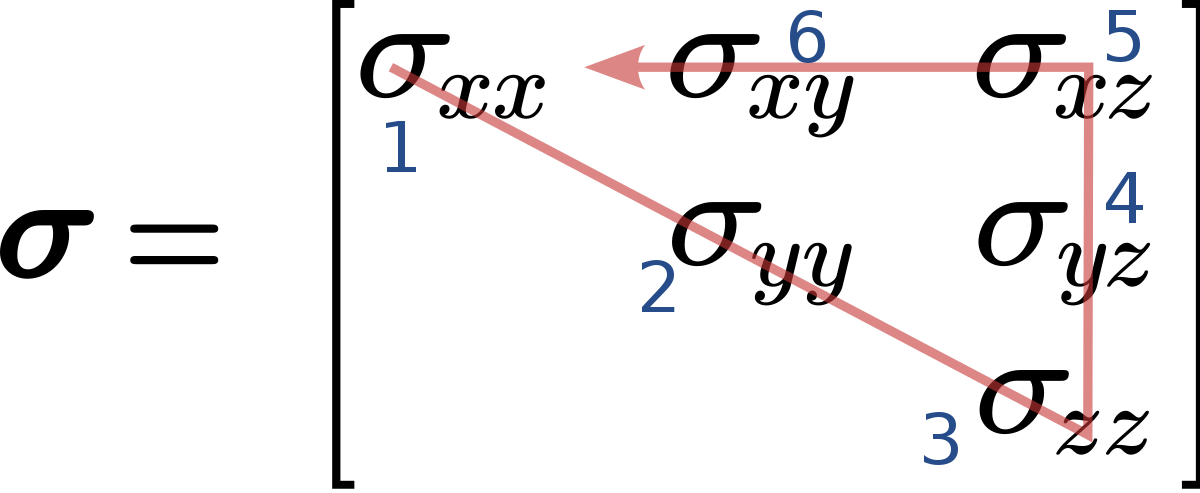
\includegraphics[width=0.5\textwidth]{Voigt_notation_Mnemonic_rule_svg.png}
    \caption{Viogt notation (From: \href{https://en.wikipedia.org/wiki/Voigt_notation}{Wiki})}
    \label{fig_voigt}
\end{figure}


\begin{lstlisting}[language=bash, caption=Source input file using discrete STF, label={lst_stf_value},
   numbers=left, numbersep=5pt,numberstyle=\tiny\color{codegray}, commentstyle=\color{codegreen},
   frame=single]
# name_of_this_input_src
evt_1_stf_value
# number of source
1
# meaning of the location: 0 computational coordinate, 1 physical coordinate
#     axis or depth of the third coordinate: 0 axis, 1 depth
0 1
# stf_input_type and time length info
#  0 4.0 : analytic and time window length of each stf
#  1 0.05 20  : 1 value and time_step num_of_step
1 0.025 40
# 1(force) 2(momoment) 3(force+moment)
#    mechanism type for moment source: 0 moment, 1 angle + mu + D + A
2 0
# meta data of each source
#   sx sy sz
80 49 50
# value data for each source
#  t0
0.0 
# Mxx etc
4.29488e+12    4.29488e+12   4.29488e+12     0.0  0.0  0.0
1.0088e+13     1.0088e+13    1.0088e+13      0.0  0.0  0.1
2.24061e+13    2.24061e+13   2.24061e+13     0.0  0.0  0.0
4.70162e+13    4.70162e+13   4.70162e+13     0.0  0.0  0.0
9.31041e+13    9.31041e+13   9.31041e+13     0.0  0.0  0.0
1.73751e+14    1.73751e+14   1.73751e+14     0.0  0.0  0.0
3.05036e+14    3.05036e+14   3.05036e+14     0.0  0.0  0.0
5.02611e+14    5.02611e+14   5.02611e+14     0.0  0.0  0.0
7.7483e+14     7.7483e+14    7.7483e+14      0.0  0.0  0.0
1.11265e+15    1.11265e+15   1.11265e+15     0.0  0.0  0.0
1.47863e+15    1.47863e+15   1.47863e+15     0.0  0.0  0.0
1.79991e+15    1.79991e+15   1.79991e+15     0.0  0.0  0.0
1.97157e+15    1.97157e+15   1.97157e+15     0.0  0.0  0.0
1.87557e+15    1.87557e+15   1.87557e+15     0.0  0.0  0.0
1.41548e+15    1.41548e+15   1.41548e+15     0.0  0.0  0.0
5.58831e+14    5.58831e+14   5.58831e+14     0.0  0.0  0.0
-6.2831e+14    -6.2831e+14   -6.2831e+14     0.0  0.0  0.0
-1.97263e+15   -1.97263e+15  -1.97263e+15    0.0  0.0  0.0
-3.22222e+15   -3.22222e+15  -3.22222e+15    0.0  0.0  0.0
-4.1098e+15    -4.1098e+15   -4.1098e+15     0.0  0.0  0.0
-4.43113e+15   -4.43113e+15  -4.43113e+15    0.0  0.0  0.0
-4.1098e+15    -4.1098e+15   -4.1098e+15     0.0  0.0  0.0
-3.22222e+15   -3.22222e+15  -3.22222e+15    0.0  0.0  0.0
-1.97263e+15   -1.97263e+15  -1.97263e+15    0.0  0.0  0.0
-6.28308e+14   -6.28308e+14  -6.28308e+14    0.0  0.0  0.0
5.58831e+14    5.58831e+14   5.58831e+14     0.0  0.0  0.0
1.41548e+15    1.41548e+15   1.41548e+15     0.0  0.0  0.0
1.87557e+15    1.87557e+15   1.87557e+15     0.0  0.0  0.0
1.97157e+15    1.97157e+15   1.97157e+15     0.0  0.0  0.0
1.79991e+15    1.79991e+15   1.79991e+15     0.0  0.0  0.0
1.47863e+15    1.47863e+15   1.47863e+15     0.0  0.0  0.0
1.11265e+15    1.11265e+15   1.11265e+15     0.0  0.0  0.0
7.7483e+14     7.7483e+14    7.7483e+14      0.0  0.0  0.0
5.02611e+14    5.02611e+14   5.02611e+14     0.0  0.0  0.0
3.05036e+14    3.05036e+14   3.05036e+14     0.0  0.0  0.0
1.73751e+14    1.73751e+14   1.73751e+14     0.0  0.0  0.0
9.3104e+13     9.3104e+13    9.3104e+13      0.0  0.0  0.0
4.70162e+13    4.70162e+13   4.70162e+13     0.0  0.0  0.0
2.24061e+13    2.24061e+13   2.24061e+13     0.0  0.0  0.0
1.0088e+13     1.0088e+13    1.0088e+13      0.0  0.0  0.0
\end{lstlisting}


\chapter*{Copyright}
\addcontentsline{toc}{chapter}{Copyright}

Main historical authors: \\

$\copyright$ October 2021\\

\noindent
This program is free software; you can redistribute it and/or modify
it under the terms of the xxx License as published 
by the Free Software Foundation (see xxx).\\

\noindent
Please note that by contributing to this code, the developer understands and agrees that this project and contribution
are public and fall under the open source license mentioned above.\\

\noindent
\textbf{\underline{Evolution of the code:}}\\


%%%%%%%%%%%%%%%%%%%%%%%%%%%%%%%%%%%%%%%%%%%%%%%%%
%% REFERENCES
%%%%%%%%%%%%%%%%%%%%%%%%%%%%%%%%%%%%%%%%%%%%%%%%%
\bibliography{citation}

%%%%%%%%%%%%%%%%%%%%%%%%%%%%%%%%%%%%%%%%%%%%%%%%%
%% APPENDIX
%%%%%%%%%%%%%%%%%%%%%%%%%%%%%%%%%%%%%%%%%%%%%%%%%

\appendix

%\include{A_reference_frame}

%%%%%%%%%%%%%%%%%%%%%%%%%%%%%%%%%%%%%%%%%%%

\end{document}
